%%%%%%%%%%%%%%%%%%%%
% MECHANICAL MODEL %
%%%%%%%%%%%%%%%%%%%%
The system under consideration is an ensemble of identically manufactured beams \(i=1,\ldots,n\) with well-known lengths \(L_i\) and rectangular cross sections with widths \(b_i\) and heights \(h_i\).
Yet the completed beams are only similar in the sense that we assume variability in the elastic moduli \(E_i\) across the ensemble, e.g.\ due to slight irregularities in the fabrication process.
For each single beam \(i\) the Young's modulus \(E_i\) is assumed to be constant along the main beam axis.
% FORWARD FORMULA
The deflections \(\perfect{v}_i(s_{i,j})\) of a simply supported beam \(i\) under a concentrated point load \(F_i\) at midspan can be easily derived in Euler-Bernoulli beam theory.
For positions \(s_{i,j}\) along the beam axis with \(0 \leq s_{i,j} \leq L_i/2\) and \(j=1,\ldots,n_i\) the deflections follow as
\begin{equation} \label{eq:PEM:Beams:AlgebraicFormula}
  \perfect{v}_i(s_{i,j}) = \frac{F_i s_{i,j} }{48 E_i I_i} \left(3 L_i^2 - 4s_{i,j}^2 \right), \;\, \text{for} \;\, 0 \leq s_{i,j} \leq L_i/2,
\end{equation}
where the moment of inertia is given as \(I_i = b_i h_i^3 / 12\).
Likewise a symmetric expression holds for positions \(s_{i,j}\) along the main axis with \(L_i/2 \leq s_{i,j} \leq L_i\).
% SIMPLY SUPPORTED BEAM
A single simply supported beam is visualized in \cref{fig:PEM:Beams:SimpleBeam}.
\begin{figure}[ht]
  \centering
  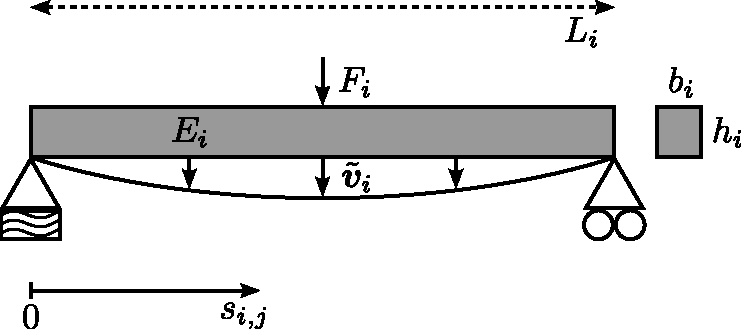
\includegraphics[width=\PEMbeamWidth]{fig_PEM_SimpleBeam}
  \caption[A simply supported beam]{A simply supported beam.}
  \label{fig:PEM:Beams:SimpleBeam}
\end{figure}
\par % VECTORIZATION
Together with its symmetric counterpart, the algebraic formula \cref{eq:PEM:Beams:AlgebraicFormula} constitutes the deterministic submodel of the system under consideration.
When a load \(F_i\) is applied to a beam \(i\) with physical dimensions \(\bm{l}_i = (L_i,b_i,h_i)\) and an elastic modulus \(E_i\),
these relations predict the deflections \(\perfect{\bm{v}}_i = (\perfect{v}_i(s_{i,1}),\ldots,\perfect{v}_i(s_{i,n_i}))\) at positions \(\bm{s}_i = (s_{i,1},\ldots,s_{i,n_i})\).
We denote this as
\begin{equation} \label{eq:PEM:Beams:ForwardModel}
  \perfect{\bm{v}}_i = \mathcal{M}(E_i,F_i,\bm{l}_i,\bm{s}_i).
\end{equation}
% UNCERTAINTY MODELS
When beam deflections are measured in three-point bending tests for each member \(i=1,\ldots,n\) in the population,
multilevel inversion allows for optimal data analysis in experimental situations where the inputs of \cref{eq:PEM:Beams:ForwardModel} are subject to uncertainty.